\chapter{cavity}

\section{Purpose}
This test case is inspired from the paper from Faure (1995)
\cite{Faure1995}where the constant viscosity and $k-\epsilon$ turbulence models
are compared to tests performed in a physical model. The Smagorinski model has
been added to TELEMAC-2D after this comparison because it proved to be more
efficient on this class of applications.

\section{Approach}
A 23 metres long and 3 metres wide channel is fed by a constant flow. The fluid
is well-mixed over the 0.43 metres depth: no stratification is present. On the
left bank of the channel is located a harbour cavity. The cavity has a
cross-section (perpendicular to the channel axis) terminating with a shallow
beach having a mild slope (see Figure \ref{fig:cavity:mesh}).

This three-dimensional configuration induces the formation of large size
eddies. Bijvelds et al. \cite{Bijvelds1997} have shown that vortices induced in
a similar harbour with constant depth are better reproduced with 3-D
simulation. In our case, a 2-D simulation is possible since the beach where
large size vortices are present is very shallow. The flow is typically unsteady
although boundary conditions are steady. The Smagorinski turbulence model is
tested on this configuration.

\subsection{Geometry and mesh}

\begin{itemize}
\item Size of the model: channel = 23 m x 3 m; cavity = 6 m x 3 m
\item Water depth at rest = 0.43 m
\end{itemize}

The mesh is dense, particularly in the cavity where the vortices take place and
on the steep junction slope between the cavity and the beach. It is made up
with quadrangles split into two triangles (see Figure \ref{fig:cavity:mesh}).

\begin{itemize}
\item 8160 triangular elements
\item 4233 nodes
\item Size range: from 0.033 to 0.34 metres
\end{itemize}

\subsection{Boundaries}

\begin{itemize}
\item Channel entrance : Q = 0.155 m${}^{3}$/s imposed
\item Channel outlet: h = 0.445 m imposed
\item Lateral boundaries: solid walls with slip condition in the channel and no-slip
condition in the cavity (see Figure \ref{fig:cavity:mesh}).
\end{itemize}

Bottom:
In order to simulate small size bottom variations, the bed is uneven.
Manning friction law with bottom roughness = 0.015
Bed isolines and a cross-section of the cavity are shown on Figure \ref{fig:cavity:mesh}.


\subsection{Physical parameters}

Turbulence: Model of Smagorinski with coefficient of Smagorinski = 0,1.

\subsection{Numerical parameters}

Type of advection:
\begin{itemize}
\item Characteristics on velocities (scheme nn$\mathrm{{}^\circ}$1)
\item conservative + modified SUPG on depth (mandatory scheme)
\end{itemize}

Type of element: Quasi-bubble triangle for velocities an linear triangle (P1) for $h$.

\begin{itemize}
\item GMRES solver
\item Accuracy = 10-3
\item Time data:
\item Time step = 0,2 sec.
\item Simulation duration = 200 sec.
\end{itemize}

\section{Results}
The velocity pattern and the free surface elevation in the cavity are shown on the figures below:
\begin{figure}
 \centering
 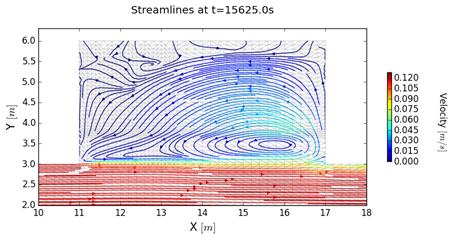
\includegraphics{img/image126}
 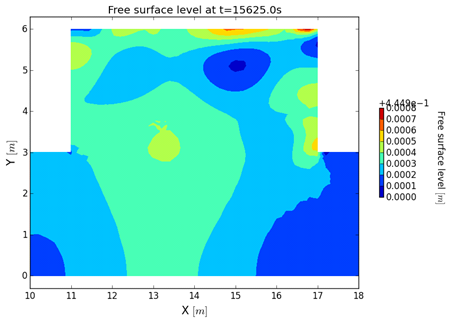
\includegraphics{img/image127}
  \caption{Velocity streamlies at final time step.}\label{fig:cavity:vel_tf}
\end{figure}


The flow is unsteady particularly in the cavity even though the boundary
conditions are steady. Great and small eddies appear and move periodically in
the cavity (see Figure  3.16 .41). The period of great eddies is longer than
the one of small eddies.

\begin{figure}
 \centering
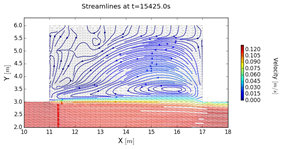
\includegraphics{img/image128}
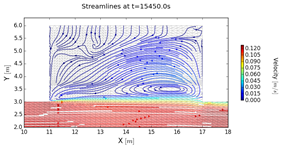
\includegraphics{img/image129}
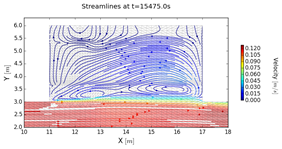
\includegraphics{img/image130}
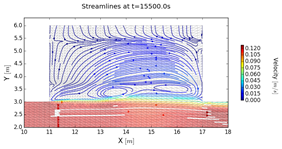
\includegraphics{img/image131}
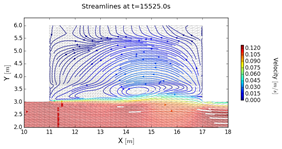
\includegraphics{img/image132}
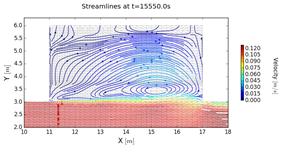
\includegraphics{img/image133}
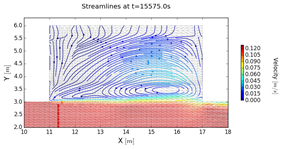
\includegraphics{img/image134}
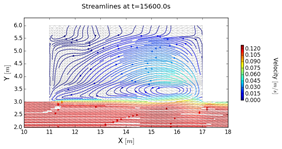
\includegraphics{img/image135}
  \caption{Evolution of the velocity field in time – Small eddy pattern.}\label{fig:cavity:evol}
\end{figure}

\section{Conclusions}
The phenomena observed on physical model are successfully reproduced by
TELEMAC-2D with the Smagorinski model, although hydrodynamics are three
dimensional in reality. In particular, the small and great eddies structures in
the cavity are well represented.

\section{Figures}
\begin{figure}
 \centering
 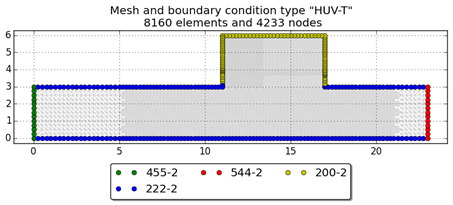
\includegraphics{img/image136}
 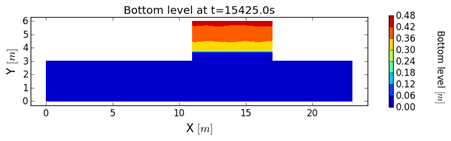
\includegraphics{img/image137}
 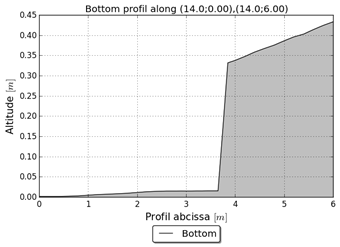
\includegraphics{img/image138}
 \caption{Mesh and topography.}\label{fig:cavity:mesh}
\end{figure}


\begin{figure}
 \centering
 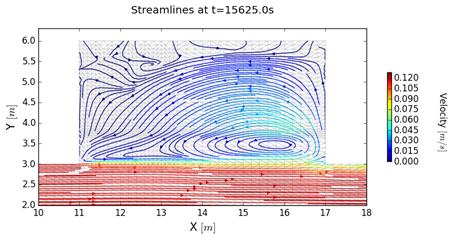
\includegraphics{img/image139}
 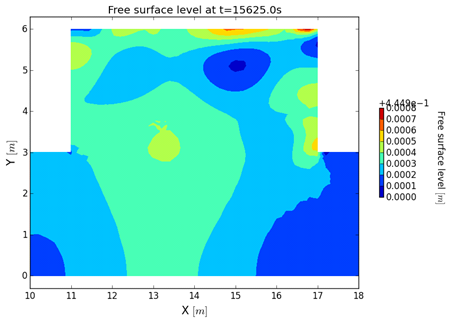
\includegraphics{img/image140}
 \caption{Velocity field and free surface in the cavity at time 15625 sec.}\label{fig:cavity:vel_prof}
\end{figure}

\begin{figure}
 \centering
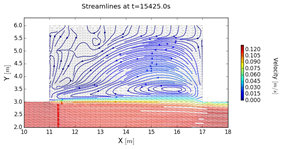
\includegraphics{img/image141}
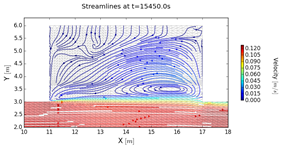
\includegraphics{img/image142}
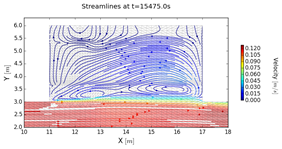
\includegraphics{img/image143}
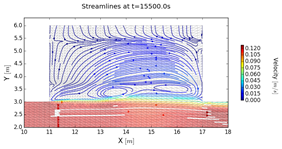
\includegraphics{img/image144}

 \caption{Evolution of the velocity field in time -- Small eddy pattern.}\label{fig:cavity:evol_small}
\end{figure}

\begin{figure}
 \centering
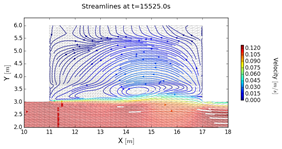
\includegraphics{img/image145}
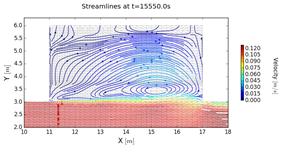
\includegraphics{img/image146}
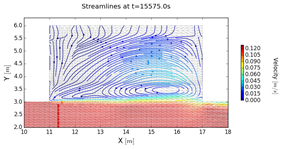
\includegraphics{img/image147}
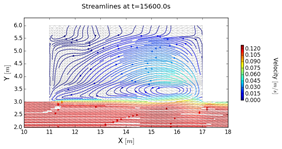
\includegraphics{img/image148}
 \caption{Evolution of the velocity field in time -- Large eddy pattern.}\label{fig:cavity:evol_large}
\end{figure}
